\documentclass[11pt,a4paper]{article}

\usepackage[utf8]{inputenc}
\usepackage[T1]{fontenc}
\usepackage[provide=*,spanish]{babel}
\usepackage{amsmath}
\usepackage{amssymb}
\usepackage{bm}
\usepackage{graphicx}
\usepackage{geometry}
\usepackage[expansion=false]{microtype}
\usepackage[hidelinks]{hyperref}

\geometry{
    top=2.5cm,
    bottom=2.5cm,
    left=2.5cm,
    right=2.5cm
}

\title{Regularización del núcleo repulsivo en el modelo de oncostreams}
\author{}
\date{}

\begin{document}

\maketitle

\section{Objetivo}

Utilizando el modelo original de Grosmann, observamos que en algunas realizaciones dos células redondas que sufren mucha presión se aproximan excesivamente hasta unirse. Este comportamiento se ve, principalmente, cuando las células elongadas se contraen ya que la condición de contracción solamente exige que se anule el movimiento en la dirección de autopropulsión, sin revisar si al volverla redonda se superpone mucho con el resto. Sin embargo, al cambiar los parámetros del sistema, vemos que esto es algo que puede pasar en otras situaciones.


Por lo tanto, veamos el origen de esto. Además, proponemos los siguientes mecanismos para evitar problemas:

\begin{enumerate}
    \item un criterio de admisibilidad para evitar que una contracción instantánea genere una superposición extrema;
    \item una regularización de la energía que introduzca un núcleo repulsivo a distancias cortas.
\end{enumerate}

\section{Interacción original}

Recordemos de mi trabajo final que llegabamos a la ecuación para la fuerza de a pares. Si llamamos:

\begin{equation}
	\mathbf C_{ij}= \left(\frac{\alpha_i + \alpha_j}{\beta_{ij}}\right)(\mathbf{I}-\mathbf{M}_{ij}),
	\label{C_ij}
\end{equation}

entonces la fuerza de a pares resulta:
\begin{equation}
	\mathbf{f}_{ij}
	=
	2 k \xi_{ij} \frac{d\mathcal{F}[\xi_{ij}]}{d\xi_{ij}}\mathbf C_{ij}  \cdot \mathbf{r}_{ij},
	\label{eq:force_general}
\end{equation}

donde, recordemos: 

\begin{itemize}
	\item $k$ es un parámetro de la fuerza.
	\item $\alpha_k=l_{\parallel, k}^{2}+l_{\perp, k}^{2}$, $\beta_{kj}=(\alpha_k+\alpha_j)^{2}-(\alpha_k \epsilon_k+\epsilon_j \alpha_j)^{2}-4\alpha_k\epsilon_k\alpha_j\epsilon_j \cos^{2}(\varphi_k-\varphi_j)$, donde $\varphi_{k, j}$ son las orientaciones y $\epsilon_k=\frac{l_{\parallel, k}^{2}-l_{\perp, k}^{2}}{l_{\parallel, k}^{2}+l_{\perp, k}^{2}}$ la excentricidad.
	\item $\mathbf{I}$ es la matriz identidad y $\mathbf{M}_{kj}=\frac{\alpha_k \epsilon_k \mathbf{Q}[\varphi_k]+\alpha_j \epsilon_j \mathbf{Q}[\varphi_j]}{\alpha_k+\alpha_j}$, con $\mathbf{Q}[\varphi_{k, j}]$ el tensor nemático.
	\item $\xi_{ij}$ es una especie de superposición normalizada entre dos células:
\end{itemize}

\begin{equation}
	\xi_{ij}
	=
	\frac{I_{ij}}{I_{ij}^{\max}}
	=
	\exp\left[
	-\mathbf r_{ij}\cdot
	\mathbf C_{ij}\cdot
	\mathbf r_{ij}
	\right],
	\label{eq:normalized_overlap}
\end{equation}

que cumple $0<\xi_{ij}\leq1$.

Acá está lo interesante, creería yo. El $\mathcal{F}[\xi_{ij}]$ es una función que aparece en la energía de intereacción binaria:

\begin{equation}
	u_{ij}
	=
	k\mathcal{F}[\xi_{ij}].
	\label{eq:energy}
\end{equation}

Según lo mismo que dice Grosmann en el paper, esta función tiene que ser una función no lineal de la variable adimensional $\xi_{ij}$. Y ellos mismos dicen que generalmente se usa $\mathcal{F}[\xi_{ij}]=\xi_{ij}^{\gamma}$ pero que se pueden usar otras formas, como implementar una dependencia en $\mathcal{F}[\xi_{ij}]$ que haga que diverja para $\xi_{ij}>\xi_{ij}^{*}$, asegurando una máxima compresibilidad. Esto último es lo que le falta al modelo, ya que ahora no tiene máxima compresibilidad (ahora lo vamos a mostrar bien).

Notemos que para el modelo original (con $\mathcal{F}[\xi_{ij}]=\xi_{ij}^{\gamma}$), obtenemos la energía:

\begin{equation}
u_{ij}^{(0)}
=
k\xi_{ij}^{\gamma},
\label{eq:original_energy}
\end{equation}

y la fuerza:

\begin{equation}
\boxed{
\mathbf f_{ij}^{(0)}
=
2k\gamma\xi_{ij}^{\gamma}
\mathbf C_{ij}\cdot\mathbf r_{ij}
}.
\label{eq:original_force}
\end{equation}

Mientras $\mathbf r_{ij} \neq \mathbf0$, esta fuerza mantiene su carácter repulsivo.

\section{Problema}

Para ver mejor el problema de esta energía que no diverge para superposiciones grandes, consideremos que dos células se aproximan a lo largo de una dirección fija:

\begin{equation}
\mathbf r_{ij}=s\hat{\mathbf n},
\end{equation}

y definamos

\begin{equation}
q_{ij}
=
\hat{\mathbf n}\cdot
\mathbf C_{ij}\cdot
\hat{\mathbf n}
>0.
\end{equation}

En esta dirección,

\begin{equation}
\xi_{ij}(s)
=
\exp\left(-q_{ij}s^2\right),
\label{eq:superposicion_direccion}
\end{equation}

y la magnitud de la fuerza original es

\begin{equation}
\left|\mathbf f_{ij}^{(0)}(s)\right|
=
2k\gamma
\left|\mathbf C_{ij}\cdot\hat{\mathbf n}\right|
s\exp\left(-\gamma q_{ij}s^2\right).
\label{eq:original_force_ray}
\end{equation}

Esta expresión se anula tanto para separaciones grandes como para centros coincidentes:

\begin{equation}
\lim_{s\rightarrow\infty}
\left|\mathbf f_{ij}^{(0)}(s)\right|
=0,
\qquad
\left|\mathbf f_{ij}^{(0)}(0)\right|
=0.
\end{equation}

Lo primero es algo que queremos pero lo segundo no.

\subsection{Máximo espacial de la fuerza}

Este problema se ve un poco mejor si vemos cuando empieza a decrecer la fuerza. Derivando la ecuación~\eqref{eq:original_force_ray} respecto de $s$,

\begin{equation}
\frac{d}{ds}
\left|\mathbf f_{ij}^{(0)}(s)\right|
\propto
\exp\left(-\gamma q_{ij}s^2\right)
\left(
1-2\gamma q_{ij}s^2
\right).
\end{equation}

Por lo tanto, la fuerza alcanza su máximo en

\begin{equation}
s_*
=
\frac{1}{\sqrt{2\gamma q_{ij}}},
\label{eq:force_peak_distance}
\end{equation}

al que corresponde la superposición (reemplaando en la ecuación \ref{eq:superposicion_direccion})

\begin{equation}
\boxed{
\xi_*
=
\exp\left(-\frac{1}{2\gamma}\right)
}.
\label{eq:force_peak_overlap}
\end{equation}

Por lo tanto,

\begin{equation}
\begin{cases}
\xi_{ij}<\xi_*:
&
\text{la fuerza aumenta cuando las células se aproximan},
\\[4pt]
\xi_{ij}>\xi_*:
&
\text{la fuerza disminuye cuando las células se aproximan}.
\end{cases}
\end{equation}

Esto nos dice que si la superposición es suficientemente alta, entonces la fuerza ya nos da problemas.

Para $\gamma=1$ y $\gamma=3$,

\begin{equation}
\xi_*(\gamma=1)
=e^{-1/2}
\simeq0.607,
\qquad
\xi_*(\gamma=3)
=e^{-1/6}
\simeq0.846.
\end{equation}

En consecuencia, para $\gamma=1$ la rama decreciente comienza a una superposición considerablemente menor que para $\gamma=3$, algo que es raro ya que parecía que $\gamma=1$ era el máximos de la fuerza. 

Las superposiciones a las que esto pasa son altas, por lo que en sistemas diluidos no parece haber problemas, pero en puntos donde la presión es muy alta, esta superposición sí se puede "vencer" y luego las células se terminan uniendo como vemos en las simulaciones.

\subsection{¿Es $\gamma=1$ más rígido?}

Recordemos que $\gamma=1$ parecía ser el máximo de la fuerza. Sin embargo, como vimos recién, la fuerza empieza a decrecer a una superposición menor que para $\gamma=3$.

Si mantenemos todo fijo en la fuerza y solamente se modifica $\gamma$, la dependencia de la fuerza es

\begin{equation}
\left|\mathbf f_{ij}^{(0)}\right|
\propto
\gamma\xi_{ij}^{\gamma}.
\end{equation}

El máximo respecto de $\gamma$ ocurre en

\begin{equation}
\gamma_*
=
-\frac{1}{\ln\xi_{ij}}.
\end{equation}

Por ejemplo, si $\xi_{ij}=e^{-1}$, la interacción es máxima para $\gamma_*=1$. Esto explica por qué $\gamma=1$ puede producir una fuerza mayor al comienzo de una colisión. No obstante, al estudiar la fuerza en función de la distancia, $\gamma=1$ entra antes en la rama decreciente. 

\subsection{Gráfico de la fuerza original}

Para poder ver gráficamente esto, pensemos en el caso de dos células redondas que se aproximan a lo largo de una dirección fija. Al ser redondas, $\mathbf{C}_{ij}$ se reduce a:

\begin{equation}
	\mathbf C_{ij}= \left(\frac{1}{4R^{2}}\right)\mathbf{I},
\end{equation}

y luego:

\begin{equation}
	q_{ij}= \frac{1}{4R^{2}},
\end{equation}

y lo mismo para $\left|\mathbf C_{ij}\cdot\hat{\mathbf n}\right|$. Entonces la ecuación \ref{eq:original_force_ray} queda (reemplazando también $s$ por $r$):

\begin{equation}
	\left|\mathbf f_{ij}^{(0)}(r)\right|
	=\frac{k\gamma}{2R^{2}}
	r\exp\left(-\frac{\gamma r^2}{4R^{2}}\right).
\end{equation}

Esta fuerza está graficada en la figura \ref{fig:gamma_dependence}. En el primer panel se ve la dependencia con $\gamma$ para una distancia fija $r=2R$, mientras que en el segundo panel se ve la dependencia con la distancia entre centros, tanto para $\gamma=1$ y $\gamma=3$.

\begin{figure}[htbp]
    \centering
    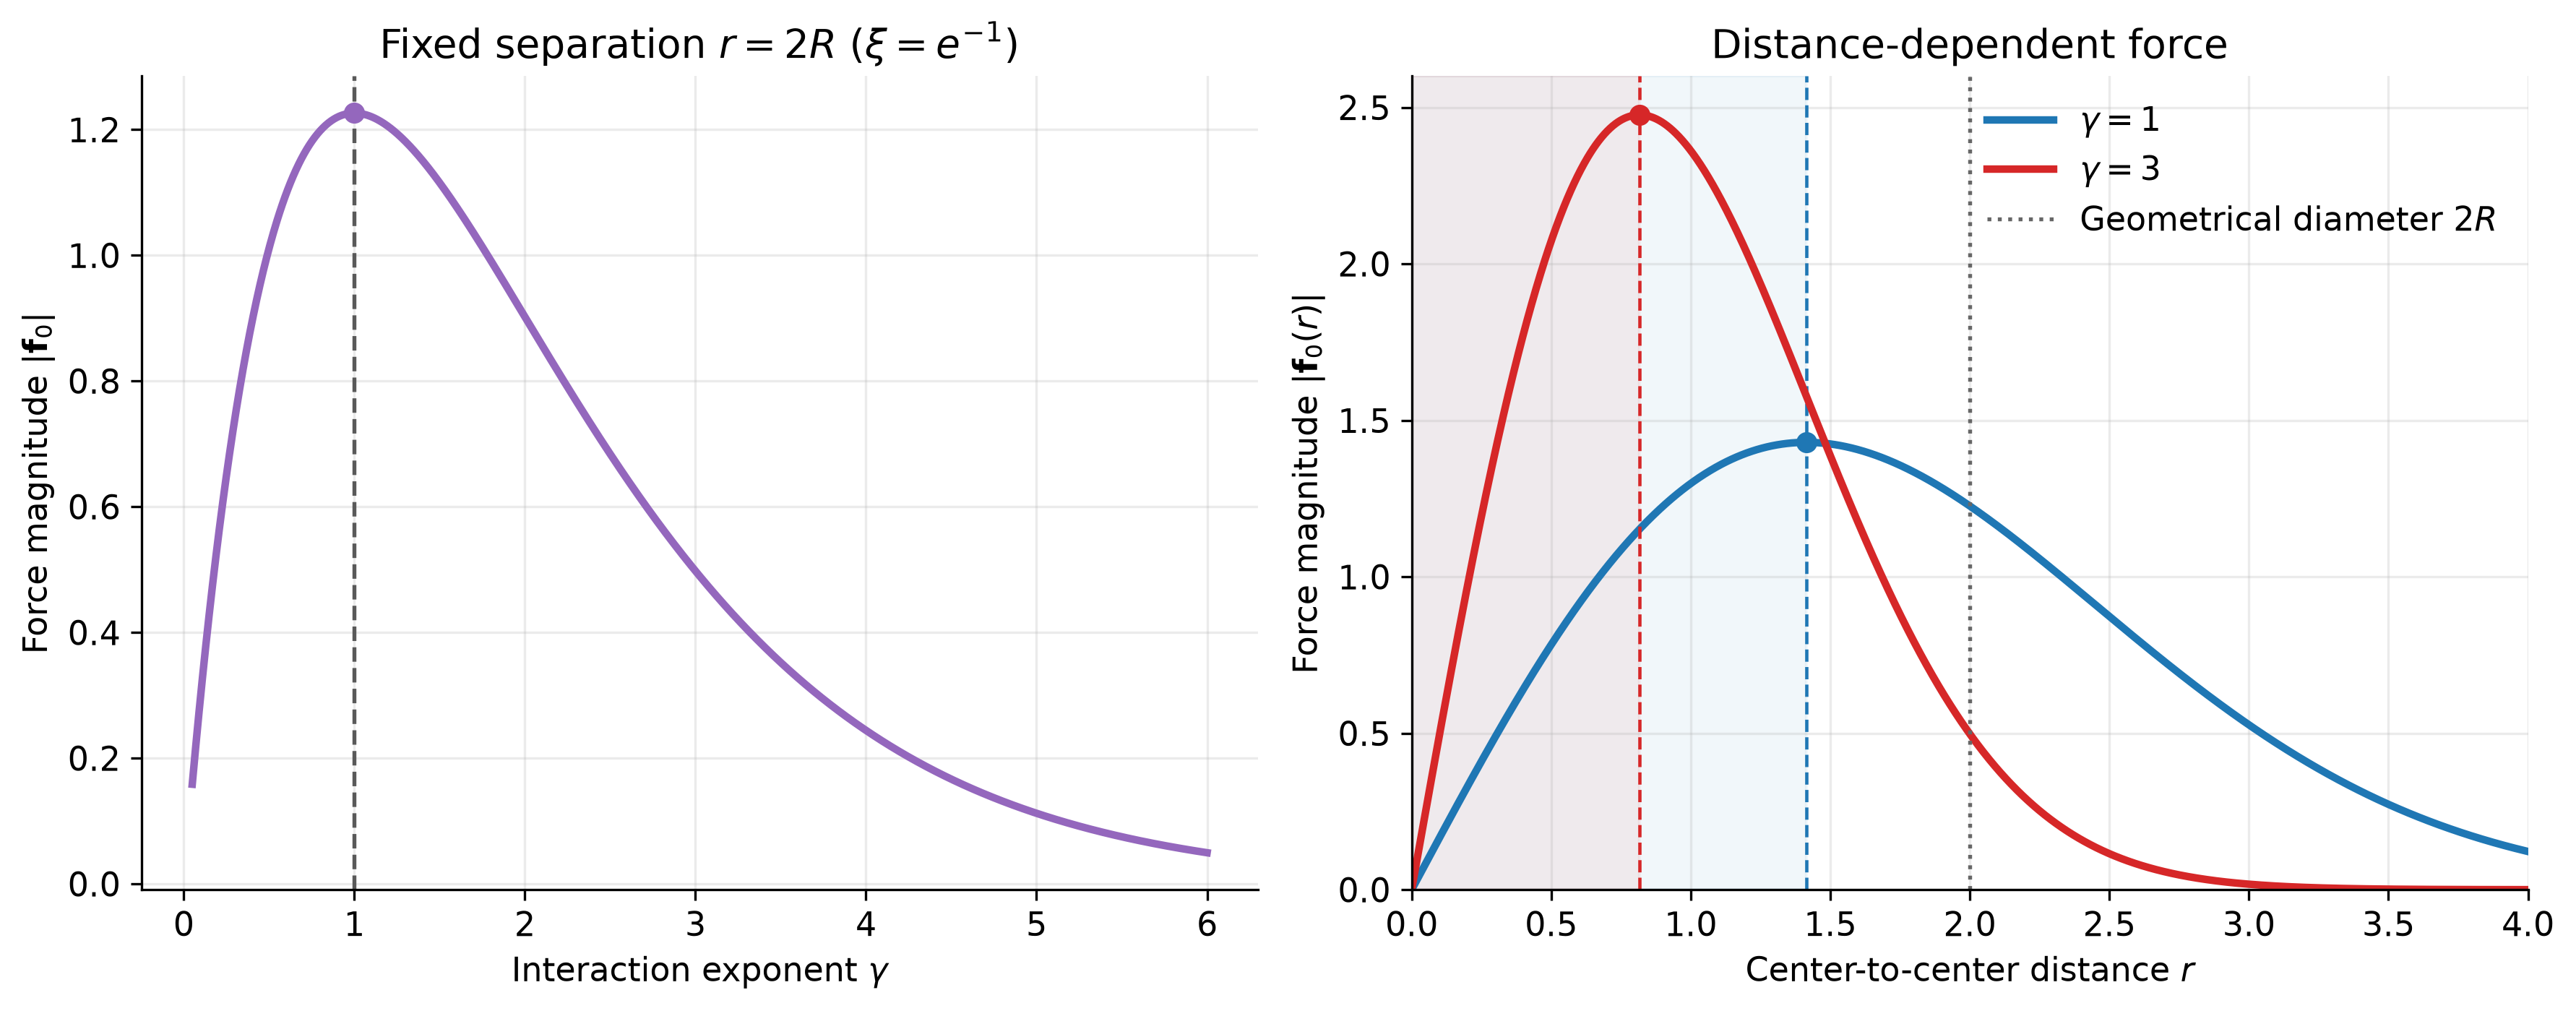
\includegraphics[width=0.96\textwidth]
    {../figures/original_force_analysis.png}
    \caption{
        Dependencia de la fuerza original con $\gamma$ (primer panel) y con la distancia (segundo panel) para dos células redondas idénticas. A distancia fija, $\gamma=1$ puede maximizar la fuerza. Sin embargo, al reducir la distancia, la fuerza termina siendo menor que para $\gamma=3$.
    }
    \label{fig:gamma_dependence}
\end{figure}

Puede verse que esta expresión también puede utilizarse para dos células elípticas idénticas y alineadas ($\varphi_i=\varphi_j$) que se aproximan a lo largo de uno de sus ejes principales comunes. En ese caso, basta reemplazar $R$ por el semieje correspondiente, $a=l_{\parallel}$ o $a=l_{\perp}$:

\begin{equation}
	\left|\mathbf f_{ij}^{(0)}(r)\right|
	=
	\frac{k\gamma}{2a^{2}}
	r\exp\left(-\frac{\gamma r^2}{4a^{2}}\right).
\end{equation}

\section{Control de las contracciones instantáneas}

Las superposiciones extremas pueden darse o por mucha presión o a partir de una contracción instantánea, ya que esta cambia la geometría de una célula elongada a una redonda, pudiendo modificar bruscamente la superposición con sus vecinas. El primer paso para "arreglar" el modelo puede ser simplemente evitar que las contracciones generen estas configuraciones.

Como ya se ha mencionado, actualmente la condición de contracción solamente exige que se anule el movimiento en la dirección de autopropulsión, sin revisar si al volverla redonda se superpone mucho con el resto. Por lo tanto, podemos agregar lo siguiente:

Si una célula elongada cumple la condición de contracción, aplicamos provisionalmente la forma redonda y calculamos:

\begin{equation}
\xi_{i}^{\mathrm{post,max}}
=
\max_{j\in\mathcal N(i)}
\left(
\xi_{ij}^{\mathrm{post}}
\right).
\end{equation}

Luego, la contracción se acepta solamente si

\begin{equation}
\boxed{
\xi_{i}^{\mathrm{post,max}}
\leq
\xi_{\mathrm{safe}}
},
\qquad
\xi_{\mathrm{safe}}<\xi_*.
\label{eq:contraction_condition}
\end{equation}

Donde $\xi_{\mathrm{safe}}$ es una superposición segura.

Para $\gamma=3$ podemos probar con

\begin{equation}
\xi_{\mathrm{safe}}=0.8
<
\xi_*
\simeq0.846.
\end{equation}

Obviamente esto no evita superposición, pero sí evita superposiciones suficientemente grandes para caer del lado decreciente de la fuerza.

Esto ayuda ya que se evitan superposiciones extremas al contraer, pero sí pueden generarse superposiciones grandes que hagan que en un sistema muy denso todavía pueda pasarse hacia el lado decreciente de la fuerza. Por lo tanto, además de este cambio, podemos ver de cambiar la elección de $\mathcal{F}[\xi_{ij}]$ (y por ende la energía de interacción).

\section{Energías propuestas}

Entonces para cambiar el funcional (o la energía), buscamos una que conserve la interacción original a superposiciones pequeñas pero diverja cuando $\xi_{ij}\rightarrow 1$. Por lo tanto, podemos proponer, dado un $0\leq\lambda\leq1$:

\begin{equation}
\boxed{
u_{ij}^{(\lambda)}
=
k\left[
(1-\lambda)\xi_{ij}^{\gamma}
-
\lambda\ln\left(1-\xi_{ij}^{\gamma}\right)
\right]
},
\label{eq:regularized_energy}
\end{equation}

Esta expresión contiene como límites

\begin{equation}
u_{ij}^{(\lambda=0)}
=k\xi_{ij}^{\gamma},
\qquad
u_{ij}^{(\lambda=1)}
=-k\ln\left(1-\xi_{ij}^{\gamma}\right).
\end{equation}

Para $\xi_{ij}\ll1$,

\begin{equation}
	-k\ln\left(1-\xi_{ij}^{\gamma}\right) \approx -k\left(\xi_{ij}+\frac{\xi_{ij}^{2}}{2}+\frac{\xi_{ij}^{3}}{3}+...\right)
\end{equation}

Por lo tanto,

\begin{equation}
u_{ij}^{(\lambda)}
=
k\xi_{ij}^{\gamma}
+
\mathcal O\left(\xi_{ij}^{2\gamma}\right),
\end{equation}

por lo que el comportamiento original se recupera como término dominante si la superposición es muy chica. En cambio, para cualquier $\lambda>0$,

\begin{equation}
\lim_{\xi_{ij}\rightarrow1}
u_{ij}^{(\lambda)}
=\infty.
\end{equation}

Para obtener la fuerza resultante, debemos calcular:
\begin{equation}
	\begin{split}
		\mathbf f_{ij}^{(\lambda)}
		&= -k\nabla_{\mathbf{r}_{ij}} \left[ (1-\lambda)\xi_{ij}^{\gamma} - \lambda\ln\left(1-\xi_{ij}^{\gamma}\right) \right] \\
		&= -k \left[ (1-\lambda)\nabla_{\mathbf{r}_{ij}}\xi_{ij}^{\gamma} - \lambda \nabla_{\mathbf{r}_{ij}} \ln\left(1-\xi_{ij}^{\gamma}\right) \right] \\
		&= -k \left[ (1-\lambda)\nabla_{\mathbf{r}_{ij}}\xi_{ij}^{\gamma} + \lambda  \frac{1}{1-\xi_{ij}^{\gamma}} \nabla_{\mathbf{r}_{ij}}\xi_{ij}^{\gamma} \right]\\
		&= -k \left[ (1-\lambda) + \lambda  \frac{1}{1-\xi_{ij}^{\gamma}}  \right]\nabla_{\mathbf{r}_{ij}}\xi_{ij}^{\gamma}\\
		&= -k \left[1 + \lambda  \frac{\xi_{ij}^{\gamma}}{1-\xi_{ij}^{\gamma}}  \right]\nabla_{\mathbf{r}_{ij}}\xi_{ij}^{\gamma}\\
	\end{split}
\end{equation}

Por lo tanto, retomando la fuerza original, tenemos que la fuerza resultante es

\begin{equation}
\boxed{
\mathbf f_{ij}^{(\lambda)}
=
\mathbf f_{ij}^{(0)}
\left[
1
+
\lambda
\frac{\xi_{ij}^{\gamma}}
{1-\xi_{ij}^{\gamma}}
\right]
}.
\label{eq:regularized_force}
\end{equation}

En la figura \ref{fig:round_regularization} se ve en el primer panel la magnitud de la fuerza para células redondas con respecto a la distancia entre centros, comparando los distintos $\lambda$. En el segundo panel se ve la corrección $\frac{f_{\lambda}}{f_0}$ para las distintas fuerzas. La corrección es pequeña cuando $\xi_{ij}^{\gamma}\ll1$, pero crece al infinito cuando se acercan. Cuanto más grande el $\lambda$, más fuerte la corrección. 

\begin{figure}[htbp]
    \centering
    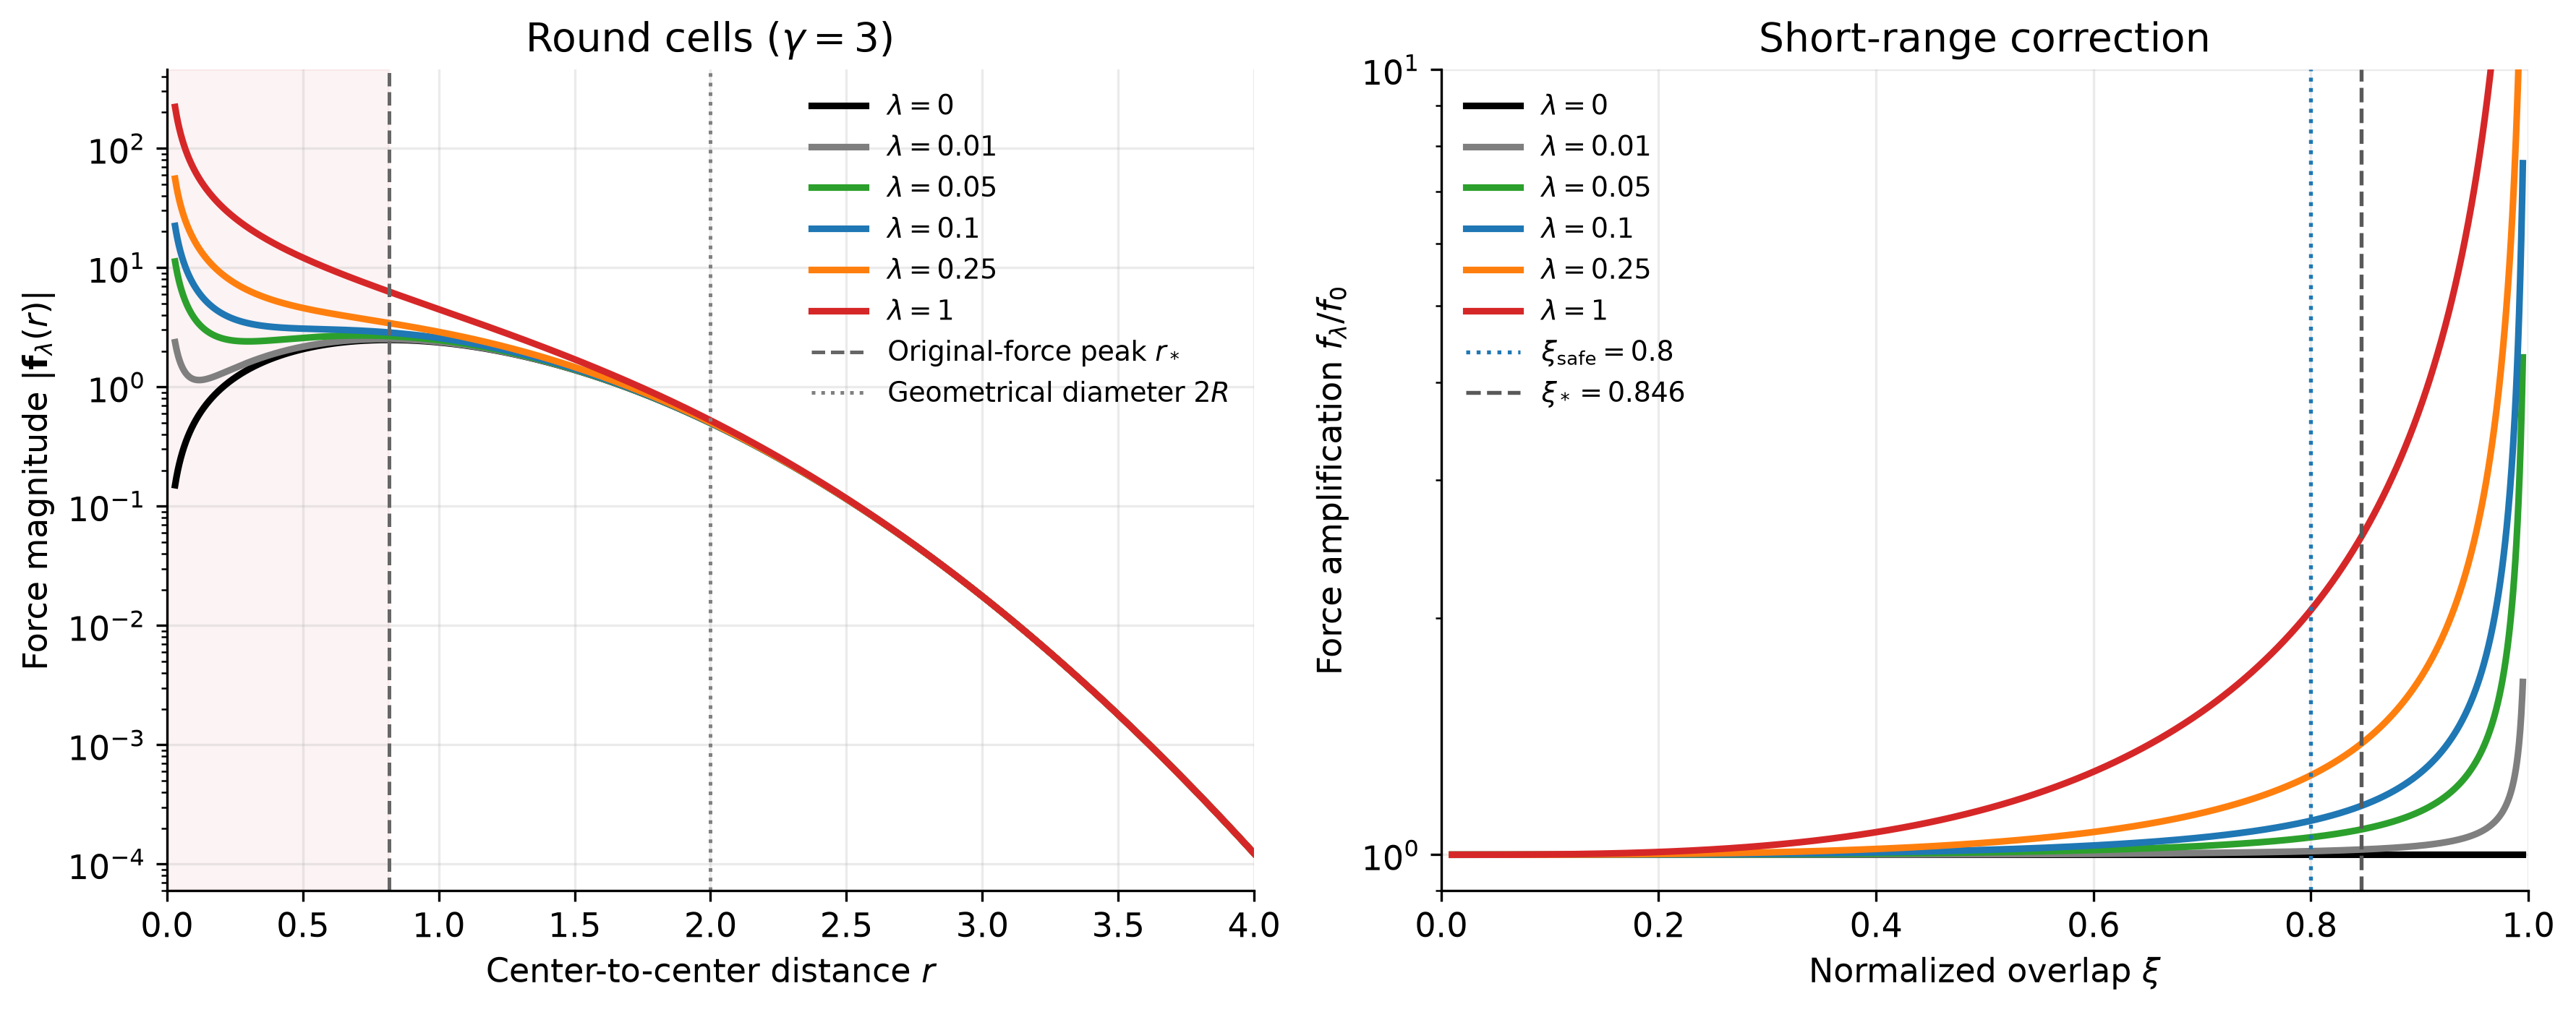
\includegraphics[width=0.96\textwidth]
    {../figures/force_regularization_analysis.png}
    \caption{
        Fuerza entre dos células redondas para diferentes valores de $\lambda$. La regularización modifica débilmente la interacción a grandes distancias y evita que la fuerza se anule a distancias cortas.
    }
    \label{fig:round_regularization}
\end{figure}

\subsection{Comportamiento a distancias cortas}

Veamos ahora cómo se comporta esta nueva fuerza a distancias cortas. Si nuevamente tomamos una dirección fija y definimos 

\begin{equation}
x
=
\gamma q_{ij}s^2.
\end{equation}

Entonces la superposición es (ecuación \ref{eq:superposicion_direccion}):

\begin{equation}
	\xi_{ij}^{\gamma}
	=e^{-x}.
\end{equation}

Entonces la magnitud de la fuerza es:

\begin{equation}
	\left|\mathbf{ f}_{ij}^{(\lambda)}(x)\right|
	= \left|\mathbf{ f}_{ij}^{(0)}(x)\right|
	\left[
	1
	+
	\lambda
	\frac{e^{-x}}
	{1-e^{-x}}
	\right].
\end{equation}

Recordando la magnitud de la fuerza original, tenemos:


\begin{equation}
	\begin{split}
		\left|\mathbf{ f}_{ij}^{(\lambda)}(x)\right|
		&= 2k\gamma
		\left|\mathbf C_{ij}\cdot\hat{\mathbf n}\right|
		\sqrt{\frac{x}{\gamma q_{ij}}} e^{-x}
		\left[
		1
		+
		\lambda
		\frac{e^{-x}}
		{1-e^{-x}}
		\right] \\
		&= 2k\gamma
		\left|\mathbf C_{ij}\cdot\hat{\mathbf n}\right|
		\sqrt{\frac{x}{\gamma q_{ij}}} e^{-x}
		\left[
		1
		+
		\lambda
		\frac{1}
		{e^{x}-1}
		\right]\\
		&= 2k\gamma
		\left|\mathbf C_{ij}\cdot\hat{\mathbf n}\right|
		\sqrt{\frac{x}{\gamma q_{ij}}} 
		\left[
		e^{-x}
		+
		\lambda
		\frac{e^{-x}}
		{e^{x}-1}
		\right].\\
	\end{split}
\end{equation}

Ahora, notemos que:

\begin{equation}
	\begin{split}
		\frac{e^{-x}}
		{e^{x}-1}
		&= \frac{1-(1-e^{-x})}
		{e^{x}-1} \\
		&= \frac{1}
		{e^{x}-1}-\frac{1-e^{-x}}
		{e^{x}-1}\\
		&= \frac{1}
		{e^{x}-1}-e^{-x}\left(\frac{e^{x}-1}
		{e^{x}-1}\right)\\
		&= \frac{1}
		{e^{x}-1}-e^{-x}\\
	\end{split}
\end{equation}

Entonces:

\begin{equation}
	\begin{split}
		\left|\mathbf{ f}_{ij}^{(\lambda)}(x)\right|
		&= 2k\gamma
		\left|\mathbf C_{ij}\cdot\hat{\mathbf n}\right|
		\sqrt{\frac{x}{\gamma q_{ij}}} 
		\left[
		e^{-x}
		+
		\lambda
		\left(\frac{1}
		{e^{x}-1}-e^{-x}\right)
		\right] \\
		&= 2k\gamma
		\left|\mathbf C_{ij}\cdot\hat{\mathbf n}\right|
		\sqrt{\frac{x}{\gamma q_{ij}}} 
		\left[
		e^{-x}(1-\lambda)
		+
		\frac{\lambda}
		{e^{x}-1}
		\right]\\
	\end{split}
\end{equation}

Es decir, si despreciamos las constantes:
\begin{equation}
	\left|\mathbf{ f}_{ij}^{(\lambda)}(x)\right|
	\propto 
	\sqrt{x} 
	\left[
	e^{-x}(1-\lambda)
	+
	\frac{\lambda}
	{e^{x}-1}
	\right].
\end{equation}

En el límite de cortas distancias, $x \rightarrow 0$ y el primer término se anula (notemos que justamente este primer término corresponde a la fuerza original, si $\lambda=0$ entonces se anula el segundo término y queda sólo este). Por otro lado, en el segundo término, $e^{x}\sim 1 + x +\mathcal{O}(x^{2})$. Por lo tanto, en el límite de distancias cortas:

\begin{equation}
	\left|\mathbf{ f}_{ij}^{(\lambda)}(x)\right|
	\propto 
	\frac{\lambda}
	{\sqrt{x}}\propto\frac{1}{s}.
\end{equation}

Por lo tanto, la fuerza deja de anularse y diverge como $1/s$.

\subsection{Criterio para elegir \texorpdfstring{$\lambda$}{lambda}}

Ahora, notemos en la figura \ref{fig:round_regularization} que pasa algo peculiar. Si $\lambda$ es muy chico, entonces se va a $\infty$ en el origen pero decrece un poco después del máximo.

Para que la fuerza aumente monótonamente cuando las células se aproximan,
debe cumplirse

\begin{equation}
\frac{d\left|\mathbf{ f}_{ij}^{(\lambda)}(x)\right|}{dx}
\leq0
\qquad
\text{para todo }x>0.
\end{equation}

Definiendo

\begin{equation}
A_{\lambda}(x)
=e^{-x}(1-\lambda)
+
\frac{\lambda}
{e^{x}-1},
\end{equation}

se tiene

\begin{equation}
\frac{d\left|\mathbf{ f}_{ij}^{(\lambda)}(x)\right|}{dx}
\propto \frac{d(\sqrt{x}A_{\lambda}(x))}{dx} =
\frac{
A_{\lambda}(x)
+2xA_{\lambda}'(x)
}{2\sqrt{x}}.
\end{equation}

El denominador es siempre positivo, por lo tanto, la condición que debemos ver es:

\begin{equation}
	H_{\lambda}(x)=A_{\lambda}(x)
	+2xA_{\lambda}'(x) \leq 0
\end{equation}

Entonces, notemos que:

\begin{equation}
	\begin{split}
		H_{\lambda}(x)
		&= A_{\lambda}(x)
		+2xA_{\lambda}'(x) \\
		&=e^{-x}(1-\lambda)
		+
		\frac{\lambda}
		{e^{x}-1} +2x\left(-e^{-x}(1-\lambda)
		-
		\frac{\lambda e^{x}}
		{(e^{x}-1)^{2}}\right)\\
		&=(1-\lambda)e^{-x}(1-2x)+ \lambda \left(\frac{1}{e^{x}-1}-\frac{2xe^{x}}{(e^{x}-1)^{2}}\right)\\
	\end{split}
\end{equation}

Acá también se ve que el primer término corresponde a la fuerza original mientras que el segundo a la corrección. De hecho, si graficamos el segundo término, vemos que es negativo $\forall x>0$. Por lo tanto, se ve que el problema de dejar de ser creciente proviene de la fuerza original. Este primer término deja de ser negativo en el rango $0<x\leq1/2$.

Como nosotros queremos que $H_{\lambda}(x) \leq 0, \forall x>0$, alcanza con ver que el máximo valor de esa función es negativo, es decir, $\max_{x} H_{\lambda}(x) \leq 0$. Pero ya sabemos que el valor máximo de $x$ tiene que estar en el rango $0<x\leq1/2$, por lo que alcanza con ver:

\begin{equation}
\max_{0<x\leq1/2}
H_{\lambda}(x)
\leq0.
\end{equation}

Entonces, podemos armar una función:

\begin{equation}
	M({\lambda})=\max_{0<x\leq1/2}
	H_{\lambda}(x),
\end{equation}

donde todos los $\lambda$ que cumplan $M(\lambda) \leq 0$ son los que cumplen que la fuerza aumenta cuando las células se acercan.

Esta función puede verse en la figura \ref{fig:monotonicity_threshold} y el punto en el que pasa a ser negativa da:

\begin{equation}
\boxed{
\lambda
\geq
\lambda_c
\simeq
0.0828
}.
\label{eq:lambda_critical}
\end{equation}

Este umbral es independiente de $\gamma$, de la relación de aspecto y de la dirección de aproximación, ya que estas cantidades solamente modifican la escala utilizada para definir $x$.

\begin{figure}[htbp]
    \centering
    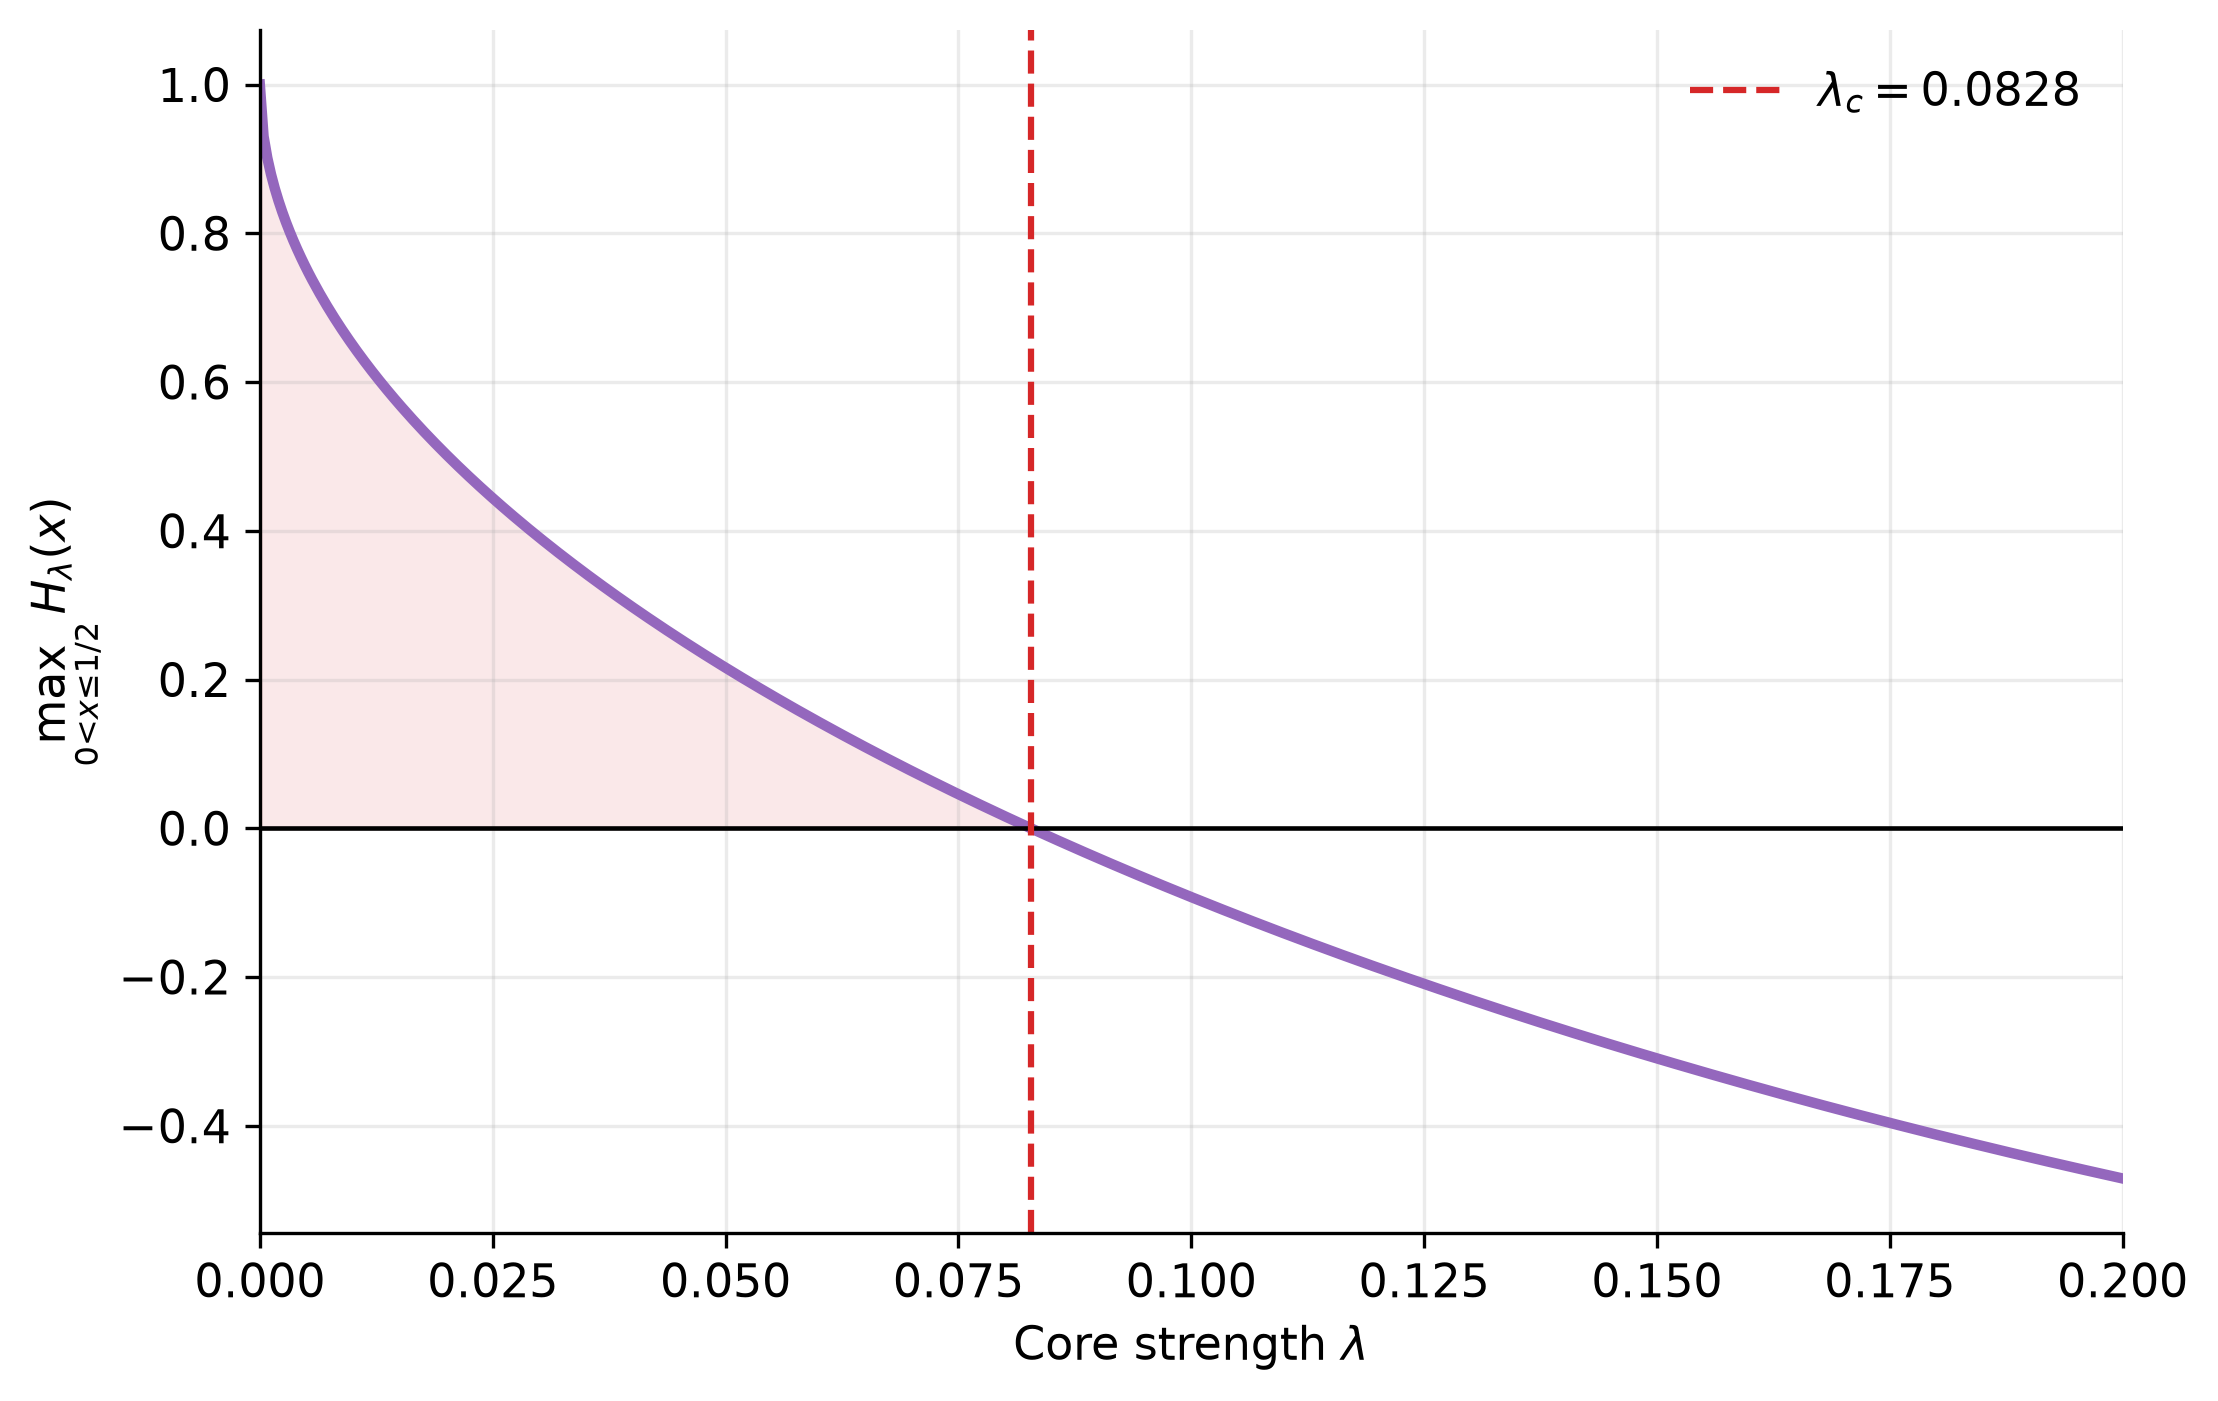
\includegraphics[width=0.70\textwidth]
    {../figures/monotonicity_analysis.png}
    \caption{
        Verificación numérica del criterio de monotonía. El cruce por
        cero de $\max_{0<x\leq1/2}[A_{\lambda}+2xA_{\lambda}']$ determina
        $\lambda_c\simeq0.0828$; para valores mayores, la fuerza aumenta
        monótonamente al aproximarse las células.
    }
    \label{fig:monotonicity_threshold}
\end{figure}


\end{document}
